\section{Behavioral revision barriers on MHST/Qwen}
\label{sec:behavior}

The primary result is a strong held-out behavioral asymmetry on MHST/Qwen. On the paired-valid test subset, committed histories require substantially more late challenger evidence to reverse than fresh histories do, with mean $\DeltaBpair = 2.78$ and 95\% CI $[2.38, 3.19]$ across $185$ valid test pairs. The full reversibility curves tell the same story: fresh histories flip earlier and more often than committed histories across the dose schedule (Figure~\ref{fig:main-behavior}A). The paired history-tax distribution is strongly right-shifted rather than being carried by a few extreme outliers (Figure~\ref{fig:main-behavior}B).

\begin{figure}[t]
    \centering
    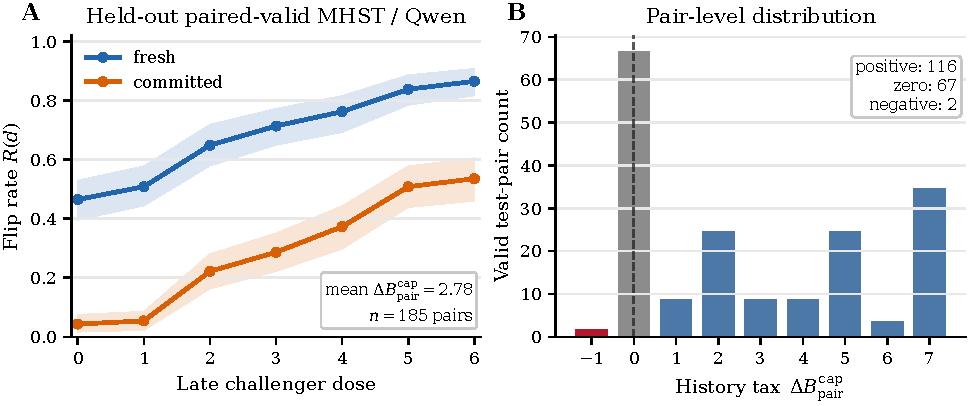
\includegraphics[width=\linewidth]{figures/figure2_main_behavior.pdf}
    \caption{Main behavioral result on held-out MHST/Qwen. \textbf{A}: reversibility curves for fresh and committed histories on the paired-valid test subset, with bootstrap confidence bands. \textbf{B}: distribution of the paired history tax $\DeltaBpair = \Bcap(\text{committed})-\Bcap(\text{fresh})$ over the same valid test pairs. Positive values dominate, showing that committed histories typically require more late challenger evidence to reverse.}
    \label{fig:main-behavior}
\end{figure}

That asymmetry is not uniform noise over the grid. It is structured by $(m,k)$, and the structure is informative. The $k{=}0$ column behaves as an exact null, while the $k{>}0$ cells carry the signal and grow with history depth (Figure~\ref{fig:controls}A). The stronger same-current-leader reading is also supported, but only on the leader-consistent subset: on held-out $\Slead$, the paired-valid mean remains same-sign at $1.85$ with 95\% CI $[1.41, 2.30]$ across $113$ valid pairs. This matters for rhetoric as much as for statistics: it licenses stronger same-current-leader wording locally, but it does not justify using that wording globally.

A separate full-curve summary confirms that the result is not carried only by the clipped barrier scalar. The paired mean-flipability-over-doses gap is $0.3969$ overall (95\% CI $[0.3420, 0.4510]$), remains same-sign on $\Slead$ at $0.2642$ (95\% CI $[0.2035, 0.3300]$), and keeps $k{=}0$ exactly null (Figure~\ref{fig:controls}B). In addition, the locked output-margin control remains same-sign under the required tertile fallback (Appendix~\ref{app:additional-controls}). Taken together, these analyses support a strong behavioral conclusion: matching designated incumbent/challenger state is not enough to determine revisability.

\begin{figure}[t]
    \centering
    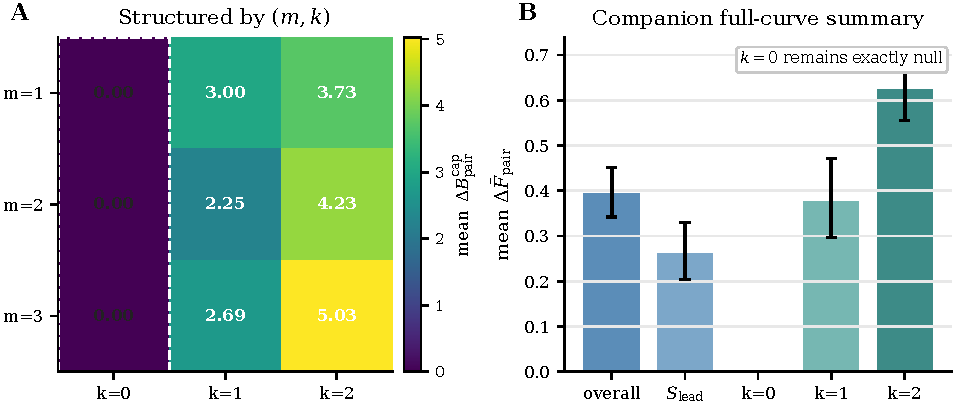
\includegraphics[width=\linewidth]{figures/figure3_control_ladder.pdf}
    \caption{Control ladder for the main MHST/Qwen result. \textbf{A}: mean paired barrier gap by $(m,k)$ on held-out test pairs; the $k{=}0$ column is exactly null, while the $k{>}0$ cells are positive. \textbf{B}: companion full-curve summary from mean flipability over doses. The overall result, the leader-consistent subset, and the $k{>}0$ cells are all same-sign; the $k{=}0$ subset remains exactly null.}
    \label{fig:controls}
\end{figure}

\begin{table}[t]
    \centering
    \small
    \begin{threeparttable}
    \caption{Main behavioral summary on held-out MHST/Qwen test pairs.}
    \label{tab:main-behavior}
    \begin{tabularx}{\linewidth}{>{\raggedright\arraybackslash}X c c c}
        \toprule
        Summary & Pairs & Mean & 95\% CI \\
        \midrule
        Paired barrier gap $\DeltaBpair$ & 185 & 2.7784 & [2.3836, 3.1893] \\
        Leader-consistent paired barrier gap & 113 & 1.8496 & [1.4071, 2.3011] \\
        Companion paired mean-flipability gap $\DeltaMeanFlip$ & 185 & 0.3969 & [0.3420, 0.4510] \\
        Leader-consistent companion gap & 113 & 0.2642 & [0.2035, 0.3300] \\
        \bottomrule
    \end{tabularx}
    \begin{tablenotes}[flushleft]
        \item The required $k{=}0$ cell is exactly null under both summaries. The output-margin control remains same-sign and satisfies the locked control rule under the tertile fallback; the corresponding plot is deferred to Appendix~\ref{app:additional-controls} to keep the behavioral core visually central.
    \end{tablenotes}
    \end{threeparttable}
\end{table}

This control ladder rules out the easiest dismissals without needing more experiments. The result is not simply generic primacy or order sensitivity: the required $k{=}0$ cells remain exactly null, the leader-consistent subset stays same-sign, and the output-margin-controlled analysis stays same-sign. It is also not just a metric trick, because both the clipped barrier summary and the independent full-curve companion summary tell the same story. The paper's main contribution is therefore already established before the internal sections begin.
